\documentclass{article}

\usepackage{graphicx}
\usepackage{tikz}
\usepackage{tikzsymbols}
\usetikzlibrary{calc,patterns,shapes.geometric}
\pagestyle{empty}
\usepackage[margin=0pt]{geometry}
\geometry{papersize={14in,12in}}

\def\centerarc[#1](#2)(#3:#4:#5){\draw[#1] ($(#2)+({#5*cos(#3)},{#5*sin(#3)})$) arc (#3:#4:#5);}

\begin{document}
	\begin{figure}
		\centering
		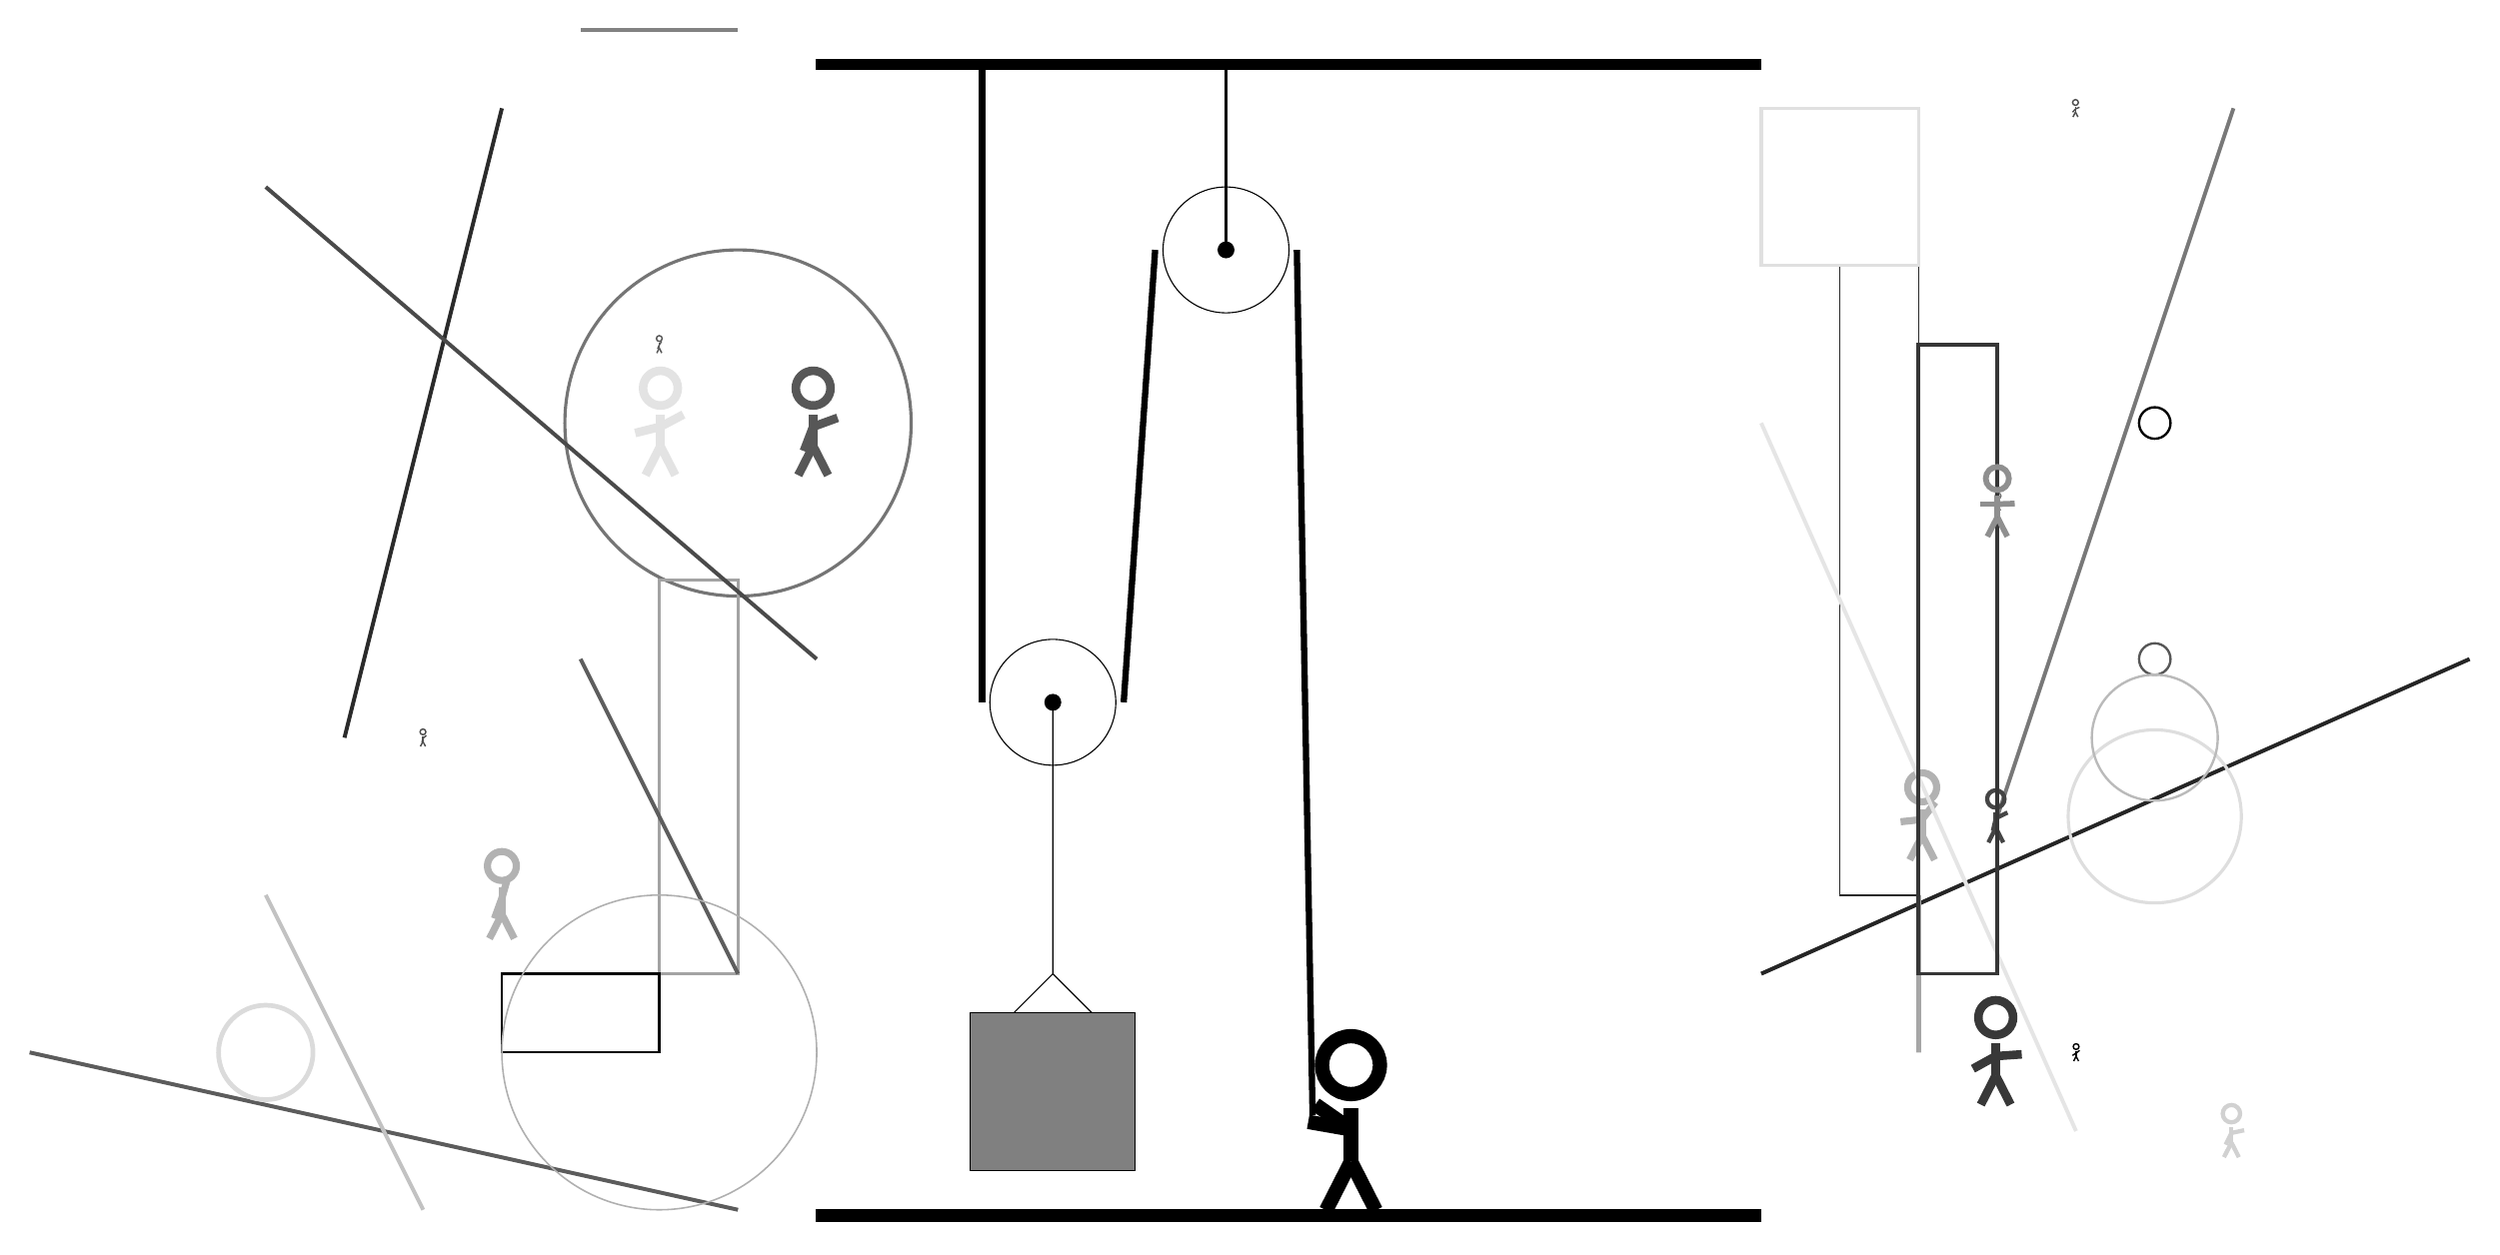
\begin{tikzpicture}
			%%%%% START %%%%%
			
			\draw[fill=black] (-2, 11.5) rectangle (10, 11.625);
			
			\draw (3.2, 9.2) circle (0.8);
			\draw[fill=black] (3.2, 9.2) circle (0.1);
			\draw[thick] (3.2, 9.2) -- (3.2, 11.5);
			
			\draw (1, 3.45) circle (0.8);
			\draw[fill=black] (1, 3.45) circle (0.1);
			
			\draw (1, 3.45) -- (1, 0.0) -- (0.5, -0.5);
			\draw (1, 0.0) -- (1.5, -0.5);
			\draw[fill=black!50] (-0.05, -0.5) rectangle (2.05, -2.5);
			
			\draw[line width=0.8mm] (0.1, 11.5) -- (0.1, 3.45);
			\centerarc[line width=0.8mm](1, 3.45)(180:360:0.9);
			\draw[line width=0.8mm](1.9, 3.45) -- (2.3, 9.2);
			\centerarc[line width=0.8mm](3.2, 9.2)(0:180:0.9);
			\draw[line width=0.8mm](4.1, 9.2) -- (4.3, -1.8);
			
			\node[line width=0.3mm, color=black!100] at (14, -1) {\Strichmaxerl[1][34][37]};
			
			\draw [line width=0.4mm, color=black!54](-3, 7) circle (2.2);
			\draw[line width=0.2mm, color=black!83] (11, 1) rectangle (12, 9);
			\draw[line width=0.5mm, color=black!85](10, 0) -- (19, 4);
			\draw[line width=0.5mm, color=black!53](13, 2) -- (16, 11);
			\draw[line width=0.5mm, color=black!83](-6, 11) -- (-8, 3);
			
			\node[line width=0.2mm, color=black!11] at (-4, 7) {\Strichmaxerl[6][14][28]};
			\draw[line width=0.4mm, color=black!36] (-3, 5) rectangle (-4, 0);
			\node[line width=0.4mm, color=black!66] at (-4, 8) {\Strichmaxerl[1][67][58]};
			\node[line width=0.7mm, color=black!69] at (-7, 3) {\Strichmaxerl[1][77][40]};
			
			\node[line width=0.4mm, color=black!56] at (13, 6) {\Strichmaxerl[1][3][74]};
			\draw[line width=0.3mm, color=black!98] (-4, 0) rectangle (-6, -1);
			\draw [line width=0.3mm, color=black!66](15, 4) circle (0.2);
			
			\draw[line width=0.5mm, color=black!64](-3, -3) -- (-12, -1);
			\node[line width=0.4mm, color=black!30] at (12, 2) {\Strichmaxerl[5][6][53]};
			\node[line width=0.7mm, color=black!73] at (13, 2) {\Strichmaxerl[3][77][26]};
			
			\draw [line width=0.4mm, color=black!13](15, 2) circle (1.1);
			
			\draw [line width=0.3mm, color=black!27](15, 3) circle (0.8);
			\draw[line width=0.5mm, color=black!63](-3, 0) -- (-5, 4);
			\draw[line width=0.7mm, color=black!35] (12, -1) rectangle (12, 1);
			\draw[line width=0.5mm, color=black!49](-5, 12) -- (-3, 12);
			
			\draw[line width=0.5mm, color=black!10](14, -2) -- (10, 7);
			\draw [line width=0.3mm, color=black!100](15, 7) circle (0.2);
			\node[line width=0.5mm, color=black!30] at (-6, 1) {\Strichmaxerl[5][70][74]};
			\node[line width=0.4mm, color=black!69] at (14, 11) {\Strichmaxerl[1][49][22]};
			\draw[line width=0.5mm, color=black!79] (12, 0) rectangle (13, 8);
			\draw [line width=0.6mm, color=black!14](-9, -1) circle (0.6);
			\draw[line width=0.5mm, color=black!24](-7, -3) -- (-9, 1);
			\node[line width=0.2mm, color=black!44] at (13, 6) {\Strichmaxerl[4][0][2]};
			\node[line width=0.2mm, color=black!66] at (-2, 7) {\Strichmaxerl[6][69][20]};
			\node[line width=0.3mm, color=black!18] at (16, -2) {\Strichmaxerl[3][64][12]};
			\draw [line width=0.2mm, color=black!31](-4, -1) circle (2.0);
			\draw[line width=0.5mm, color=black!71](-2, 4) -- (-9, 10);
			
			\draw[line width=0.4mm, color=black!12] (12, 9) rectangle (10, 11);
			\node[line width=0.4mm, color=black!78] at (13, -1) {\Strichmaxerl[6][29][4]};
			
			\node at (4.7, -1.9) {\Strichmaxerl[10][-35][170]};
			
			\draw[fill=black] (-2, -3) rectangle (10, -3.15);
			
			%%%%% END %%%%%
		\end{tikzpicture}
	\end{figure}	
\end{document}